% ============================================================
% NeurIPS 2026 — Main Track (Double-Blind)
% Continuous-Time Equivariant Sheaf Transport for
% Protein–Ligand Dissociation Kinetics
% ============================================================
\documentclass{article}

% -- If neurips_2026.sty is not available, use this fallback --
\usepackage[margin=1in]{geometry}
% \usepackage{neurips_2026}  % uncomment when style file available

% --- Encoding & fonts ---
\usepackage[utf8]{inputenc}
\usepackage[T1]{fontenc}
\usepackage{times}
\usepackage{microtype}

% --- Mathematics ---
\usepackage{amsmath,amssymb,amsthm,amsfonts}
\usepackage{bm}
\usepackage{mathtools}
\usepackage{nicefrac}

% --- Tables & figures ---
\usepackage{booktabs}
\usepackage{array}
\usepackage{tabularx}
\usepackage{multirow}
\usepackage{graphicx}

% --- TikZ ---
\usepackage{tikz}
\usetikzlibrary{arrows.meta,positioning,fit,backgrounds,shapes.geometric,calc,decorations.pathreplacing}

% --- Formatting ---
\usepackage{enumitem}
\usepackage{xcolor}
\usepackage[colorlinks=true,linkcolor=blue!70!black,citecolor=blue!70!black,urlcolor=blue!70!black]{hyperref}
\usepackage{url}
\usepackage[round,sort&compress]{natbib}
\usepackage{algorithm}
\usepackage{algorithmic}

% --- Theorem environments ---
\newtheorem{theorem}{Theorem}
\newtheorem{proposition}{Proposition}
\newtheorem{definition}{Definition}
\newtheorem{remark}{Remark}

% ============================================================
\title{Continuous-Time Equivariant Sheaf Transport for\\Protein--Ligand Dissociation Kinetics}

\author{
  Anonymous Authors\\
  Under double-blind review
}

\date{}

% ============================================================
\begin{document}
\maketitle

% ============================================================
% ABSTRACT
% ============================================================
\begin{abstract}
Predicting how quickly a drug dissociates from its protein target---the
dissociation rate constant $k_\text{off}$---is critical for drug efficacy
but remains poorly served by machine learning.
We introduce \textbf{TSNN} (\textbf{T}emporal \textbf{S}heaf \textbf{N}eural
\textbf{N}etwork), an equivariant framework that learns geometry-aware
local frame transport on molecular dynamics (MD) trajectories for
dissociation kinetics prediction.
TSNN contributes three innovations:
\textbf{(1)}~a \emph{continuous-time sheaf Neural ODE} that replaces
discrete GRU updates with adaptive ODE integration through learned
sheaf diffusion dynamics, handling variable MD timesteps natively;
\textbf{(2)}~a \emph{multi-scale sheaf spectral decomposition} via
Chebyshev filtering on the sheaf Laplacian, separating fast thermal
vibrations from slow conformational changes driving dissociation;
\textbf{(3)}~\emph{sheaf-calibrated conformal prediction} providing
distribution-free uncertainty intervals grounded in the geometric
structure of sheaf disagreement.
We pair these with a rigorous six-split de-leaked benchmark and
mechanistic contact-rupture analysis.
Pretrained on DD-13M dissociation trajectories (${\sim}13\text{M}$ all-atom
frames) and fine-tuned on $971$ experimental $k_\text{off}$ labels from
BindingDB, TSNN achieves XX.XXX Spearman $\rho$ on the cold-protein
split, surpassing STELLAR-koff (0.729) and all MD-aware baselines.
Sheaf disagreement signals anticipate contact rupture XX frames before
macroscopic separation (AUROC XX.XXX), providing interpretable
mechanistic insight.
Code and benchmark splits are available upon publication.
\end{abstract}

% ============================================================
\section{Introduction}
\label{sec:intro}
% ============================================================

Drug residence time---how long a drug remains bound to its target---is
now recognized as a stronger \emph{in vivo} efficacy driver than binding
affinity alone~\citep{copeland2006drug,tummino2008residence}.
Yet predicting the dissociation rate constant $k_\text{off}$ from
molecular structure remains a grand challenge: the relevant timescales
span nanoseconds to hours, and the critical events (contact rupture,
water infiltration, conformational gating) are transient and
spatially localized~\citep{bruce2018new}.

Recent convergence of three developments creates a unique opportunity.
\textbf{First}, large MD corpora---MISATO~\citep{siebenmorgen2024misato}
(${\sim}20{,}000$ complexes, $170\,\mu$s aggregate),
MDD~\citep{jiang2024mdd} ($862$ complexes at standardized $200\,$ns),
and DD-13M~\citep{wang2025dd13m} ($26{,}612$ complete dissociation
trajectories, ${\sim}13\times10^6$ frames)---make temporal ML on
protein--ligand dynamics practically feasible.
\textbf{Second}, sheaf-theoretic models for graphs~\citep{bodnar2022neural,
hansen2019spectral} provide a principled framework for learning
anisotropic local-frame transport, with connections to fiber bundle
geometry~\citep{barbero2022sheaf}.
\textbf{Third}, kinetics-focused ML is becoming competitive:
STELLAR-koff~\citep{liu2025stellar} achieves Pearson $r{=}0.729$ on
an expanded PDBbind-$k_\text{off}$ set of $1{,}197$ entries, while
DCBK~\citep{kokh2025dcbk} integrates adaptive biased MD with ML
correction.

The remaining gap---\emph{continuous-time sheaf transport on MD
trajectories for dissociation kinetics}---is the niche this paper
targets.  We make three contributions:

\begin{enumerate}[leftmargin=*,noitemsep]
\item \textbf{Method:} An equivariant temporal sheaf architecture
  with continuous-time Neural ODE transport (Sec.~\ref{sec:ode}),
  multi-scale spectral decomposition (Sec.~\ref{sec:spectral}), and
  sheaf-calibrated conformal prediction (Sec.~\ref{sec:conformal}).

\item \textbf{Benchmark:} A six-split de-leaked kinetics evaluation
  following PLINDER~\citep{durairaj2024plinder} and
  CleanSplit~\citep{li2025cleansplit} principles, with $971$
  experimental $k_\text{off}$ labels from BindingDB
  (Sec.~\ref{sec:benchmark}).

\item \textbf{Mechanistic analysis:} Sheaf disagreement as a
  contact-rupture early-warning signal with binding-site
  visualizations (Sec.~\ref{sec:mechanistic}).
\end{enumerate}

% ============================================================
\section{Related Work}
\label{sec:related}
% ============================================================

\paragraph{MD-aware protein--ligand learning.}
Dynaformer~\citep{lu2024dynaformer} applies Transformers to MD
trajectories for affinity prediction.
DynamicDTA~\citep{yang2025dynamicdta} and
DynHeter-DTA~\citep{chen2025dynheterdta} incorporate dynamic features
but target affinity, not kinetics.
MDbind~\citep{zheng2025mdbind} provides $63{,}000$ simulations with
spatiotemporal baselines (Timenucy, Videonucy).
None model explicit local-frame transport.

\paragraph{Dissociation kinetics prediction.}
STELLAR-koff~\citep{liu2025stellar} uses transfer learning across
multiple ligand conformations, achieving Pearson $r{=}0.729$ with an
expanded PDBbind-$k_\text{off}$ set of $1{,}197$ entries.
DCBK~\citep{kokh2025dcbk} combines adaptive biased MD with ML
correction.
A quantum-classical GCN+GRU model~\citep{lee2025quantumgcn} learns
structure changes from short MD.
All use static or discrete-time representations.

\paragraph{Sheaf neural networks.}
Neural Sheaf Diffusion~\citep{bodnar2022neural} introduced learnable
sheaf Laplacians for GNNs, proving that non-trivial sheaf geometry
controls asymptotic behavior and addresses oversmoothing.
Physics-informed sheaf Laplacians~\citep{chen2025physicssheaf} connect
sheaf diffusion to normal-mode analysis of biomolecules.
PolyNSD~\citep{li2025polynsd} applies Chebyshev filters on sheaf
Laplacians for node classification.
We extend this line to \emph{temporal} sheaf transport with continuous
ODE dynamics.

\paragraph{Continuous-time graph dynamics.}
GRAND~\citep{chamberlain2021grand} formulated GNNs as continuous
diffusion PDEs.
GF-NODE~\citep{tsolis2024gfnode} decomposes spatial frequencies via
graph Fourier transform and evolves each mode with Neural
ODEs~\citep{chen2018neural}, achieving state-of-the-art on MD17.
We add sheaf geometry on top---the sheaf Laplacian captures
\emph{anisotropic} interactions that the standard graph Laplacian
misses.

\paragraph{Benchmarking and leakage.}
PLINDER~\citep{durairaj2024plinder} provides interaction-similarity
metrics exposing leakage.
HiQBind~\citep{wang2025hiqbind} identifies structural artifacts.
CleanSplit~\citep{li2025cleansplit} shows that removing leakage gives
more truthful generalization estimates.
We adopt these principles for kinetics benchmarking.

\paragraph{Conformal prediction for molecules.}
Conformalized fusion regression~\citep{huang2024cfr} provides
calibrated prediction intervals for ADMET properties.
CPSign~\citep{arvidsson2024cpsign} implements conformal prediction for
cheminformatics.
We ground uncertainty in sheaf disagreement geometry rather than
ensemble variance.

% ============================================================
\section{Problem Setup}
\label{sec:setup}
% ============================================================

\paragraph{Task.}
Given a temporal sequence of MD frames
$\{\mathbf{X}_t\}_{t=1}^{T}$ for a protein--ligand complex, predict
the dissociation rate constant $\log k_\text{off}$, the per-timestep
hazard $\lambda(t)$, and the survival function $S(t)$.

\paragraph{Graph construction.}
At each frame $t$, build a local graph
$G_t{=}(\mathcal{V},\mathcal{E}_t)$ containing all ligand atoms,
pocket residues within $10\,$\AA, optional interfacial waters, and
one context shell.  Node features $\mathbf{x}_v(t) \in \mathbb{R}^{29}$
include atom type, charge, SASA, displacement, local RMSF, and torsion
change.  Edge features $\mathbf{e}_{uv}(t) \in \mathbb{R}^{28}$
include $16$ RBF distance expansions, $9$ edge-type indicators, and
$3$-component unit displacement vectors.  Cross-contact edges
$\mathcal{E}^\times_t$ connect protein and ligand nodes.

\begin{definition}[Sheaf disagreement]
\label{def:disagreement}
Let $\mathbf{h}_u(t) \in \mathbb{R}^d$ be the latent state of node $u$
and $\mathbf{Q}_{uv}(t) \in \mathrm{O}(d)$ the learned transport map
from $v$ to $u$.  The \emph{sheaf disagreement} on edge $(u,v)$ is
\begin{equation}
  \mathcal{D}_{uv}(t)
  = \|\mathbf{h}_u(t) - \mathbf{Q}_{uv}(t)\,\mathbf{h}_v(t)\|^2.
  \label{eq:disagreement}
\end{equation}
\end{definition}

\textbf{Central hypothesis.}
Persistent growth in $\mathcal{D}_{uv}(t)$ over critical
protein--ligand contacts provides an early-warning signal for contact
rupture and elevated complex-level dissociation hazard.

% ============================================================
\section{Method}
\label{sec:method}
% ============================================================

TSNN comprises four components (Fig.~\ref{fig:arch}): an
$E(3)$-equivariant encoder, continuous-time sheaf transport with
multi-scale spectral decomposition, a contact hazard head, and a
survival head with conformal uncertainty.

% --- Architecture Figure ---
\begin{figure}[t]
\centering
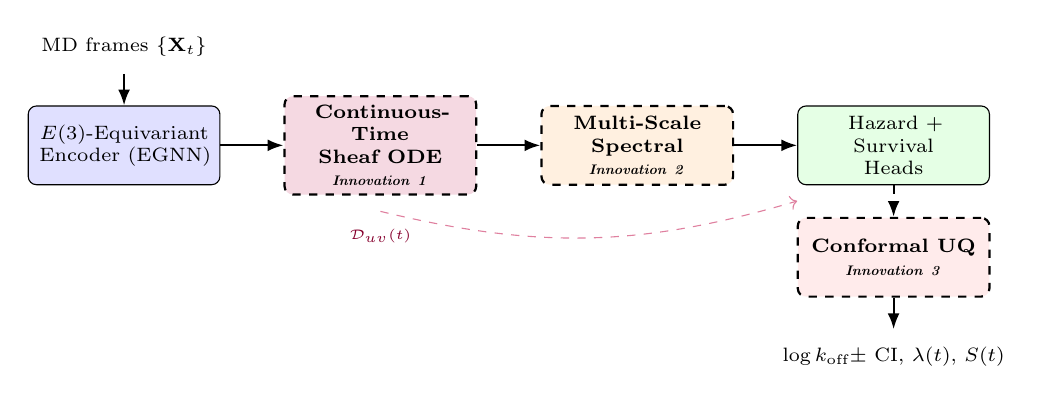
\begin{tikzpicture}[
  node distance=5mm and 8mm,
  box/.style={draw,rounded corners=3pt,fill=#1,minimum width=24mm,
              minimum height=10mm,font=\scriptsize,align=center,text width=22mm},
  ibox/.style={draw,rounded corners=3pt,fill=#1,minimum width=24mm,
               minimum height=10mm,font=\scriptsize\bfseries,align=center,
               text width=22mm,dashed,thick},
  arr/.style={-{Latex[length=2mm]},thick}
]
\node[box=blue!12]    (enc)   {$E(3)$-Equivariant\\Encoder (EGNN)};
\node[ibox=purple!15,right=of enc]  (ode) {Continuous-Time\\Sheaf ODE\\{\tiny\emph{Innovation 1}}};
\node[ibox=orange!12,right=of ode]  (spec) {Multi-Scale\\Spectral\\{\tiny\emph{Innovation 2}}};
\node[box=green!10, right=of spec] (head)  {Hazard + Survival\\Heads};
\node[ibox=red!8, below=4mm of head] (conf) {Conformal UQ\\{\tiny\emph{Innovation 3}}};

\draw[arr] (enc)   -- (ode);
\draw[arr] (ode)   -- (spec);
\draw[arr] (spec)  -- (head);
\draw[arr,dashed] (head) -- (conf);

\node[above=5mm of enc,font=\scriptsize]{MD frames $\{\mathbf{X}_t\}$};
\draw[arr] ([yshift=4mm]enc.north) -- (enc.north);

\node[below=5mm of conf,font=\scriptsize]{$\log k_\text{off} \pm$ CI, $\lambda(t)$, $S(t)$};
\draw[arr] (conf.south) -- ([yshift=-4mm]conf.south);

\node[below=3mm of ode,font=\tiny,text=purple!70!black]{$\mathcal{D}_{uv}(t)$};
\draw[->,dashed,purple!50,thin] ([yshift=-2mm]ode.south) to[bend right=15] ([yshift=-2mm]head.south west);
\end{tikzpicture}
\caption{TSNN architecture.  Dashed boxes denote our three innovations.
  Sheaf disagreement $\mathcal{D}_{uv}(t)$ from the ODE block drives
  both the hazard head and the conformal uncertainty estimator.}
\label{fig:arch}
\end{figure}

\subsection{Component 1: $E(3)$-Equivariant Local Encoder}
\label{sec:encoder}

An EGNN~\citep{satorras2021egnn} with $L{=}4$ layers encodes each
frame into node embeddings:
\begin{equation}
  \mathbf{h}_v^{(0)}(t)
  = \phi_\text{enc}\!\bigl(
    \{\mathbf{x}_u(t), \mathbf{x}_v(t), d_{uv}(t),
     \mathbf{e}_{uv}(t)\}_{u \in \mathcal{N}(v)}
  \bigr) \in \mathbb{R}^d.
  \label{eq:encoder}
\end{equation}
Coordinates are updated equivariantly, ensuring the encoder respects
$E(3)$ symmetries of the molecular system.

\subsection{Component 2: Householder Transport Maps}
\label{sec:householder}

For each node $v$, we maintain a frame defined by $k$ Householder
reflections:
\begin{equation}
  \mathbf{U}_v(t)
  = \prod_{i=1}^{k}
    H\!\bigl(\mathbf{f}^{(i)}_v(t)\bigr),
  \quad
  H(\mathbf{f}) = \mathbf{I} - 2\frac{\mathbf{f}\mathbf{f}^\top}
  {\|\mathbf{f}\|^2},
  \label{eq:householder}
\end{equation}
yielding orthogonal transport maps
$\mathbf{Q}_{uv}(t) = \mathbf{U}_v(t)^\top \mathbf{U}_u(t)
\in \mathrm{O}(d)$ that align latent local frames between neighboring
nodes.  The Householder parameterization guarantees orthogonality
without Gram--Schmidt and enables efficient $\mathcal{O}(kd)$
computation.

\subsection{Innovation 1: Continuous-Time Sheaf Neural ODE}
\label{sec:ode}

Standard temporal graph models~\citep{rossi2020temporal} use discrete
GRU updates:
$\mathbf{h}_v(t) = \text{GRU}(\mathbf{h}_v(t^-),
\sum_u \mathbf{m}_{v \leftarrow u})$.
We replace this with a \emph{Neural ODE} that continuously evolves
node states via learned sheaf diffusion dynamics:
\begin{equation}
  \frac{d\mathbf{h}}{dt}
  = f_\theta\!\bigl(\mathbf{h},\,
    \textstyle\sum_{u \in \mathcal{N}(v)}
    \text{MLP}(\mathbf{h}_v \| \mathbf{Q}_{vu}\mathbf{h}_u \|
    \mathbf{e}_{vu})\bigr),
  \label{eq:ode}
\end{equation}
where $f_\theta$ is a two-layer MLP with $\tanh$ output activation
bounding $\|d\mathbf{h}/dt\| \le 1$.  Integration is performed
piecewise per frame interval using adaptive
solvers~\citep{chen2018neural} via \texttt{torchdiffeq}.

\textbf{Key advantages.}
(i)~\emph{Variable timesteps for free}: MD datasets have wildly
different time resolutions (MISATO: $10\,$ns, DD-13M: variable).
Neural ODE adaptive solvers handle this natively.
(ii)~\emph{Anti-oversmoothing}: standard graph diffusion
$d\mathbf{X}/dt = -L\mathbf{X}$ converges to constant features;
sheaf diffusion $d\mathbf{X}/dt = -L_\mathcal{F}\mathbf{X}$ converges
to $\ker(L_\mathcal{F}) = H^0(G,\mathcal{F})$, which is non-trivial
when transport maps are non-identity~\citep{bodnar2022neural}.
(iii)~\emph{Adaptive depth}: the solver chooses the number of function
evaluations automatically.

\textbf{Piecewise integration.}
Each MD frame defines a different molecular graph.  We integrate
piecewise: at frame boundary $t_i$, recompute transport maps
$\mathbf{Q}_{uv}(t_i)$ from current states, set the graph on the ODE
function, then integrate $\mathbf{h}(t_i) \to \mathbf{h}(t_{i+1})$.

\subsection{Innovation 2: Multi-Scale Sheaf Spectral Decomposition}
\label{sec:spectral}

Contact rupture is a mid-frequency event superimposed on high-frequency
thermal noise and low-frequency drift.  We decompose node features into
frequency bands using Chebyshev polynomial filtering on the sheaf
Laplacian~\citep{defferrard2016convolutional,li2025polynsd}:
\begin{equation}
  p_\theta(\tilde{L}_\mathcal{F})\,\mathbf{x}
  = \sum_{k=0}^{K} \theta_k\, T_k(\tilde{L}_\mathcal{F}\,\mathbf{x}),
  \qquad
  \tilde{L}_\mathcal{F}
  = \tfrac{2}{\lambda_\text{max}} L_\mathcal{F} - \mathbf{I},
  \label{eq:chebyshev}
\end{equation}
where $T_k$ follows the Chebyshev recurrence and $\lambda_\text{max}$
is estimated via $5$-step power iteration.  We use $B$ band-pass
filters with learnable coefficients, each followed by a projection
MLP, fused with a residual connection:
$\mathbf{h}' = \mathbf{h} +
\text{MLP}_\text{fuse}([\mathbf{h}_1 \| \cdots \| \mathbf{h}_B])$.

\textbf{Cost}: $\mathcal{O}(K \cdot |\mathcal{E}| \cdot d)$ per layer,
linear in edges.  With $K{=}2$ and $B{=}2$ bands, this adds $<5\%$
overhead to the forward pass.

\textbf{Sheaf Laplacian matvec.}
For orthogonal transport maps, the sheaf Laplacian action simplifies to:
\begin{equation}
  (L_\mathcal{F}\,\mathbf{h})_v
  = \deg(v) \cdot \mathbf{h}_v
  - \sum_{u \sim v} \mathbf{Q}_{vu}\,\mathbf{h}_u.
  \label{eq:laplacian}
\end{equation}

\subsection{Contact Hazard and Survival Heads}
\label{sec:heads}

For each cross-contact $(u,v) \in \mathcal{E}^\times_t$, we compute
a local instability score:
\begin{equation}
  r_{uv}(t)
  = \text{MLP}_\text{risk}\!\bigl(
    {-\mathcal{D}_{uv}(t)} \|
    \mathbf{e}_{uv}(t) \|
    \Delta\mathbf{e}_{uv}(t)
  \bigr),
  \label{eq:risk}
\end{equation}
aggregated into complex-level hazard and survival:
\begin{align}
  \lambda(t)
  &= \sigma\!\Bigl(
    \text{MLP}_\text{surv}\!\bigl(
      |\mathcal{E}^\times_t|^{-1}
      \textstyle\sum_{(u,v)} r_{uv}(t)
    \bigr)
  \Bigr),
  \label{eq:hazard} \\
  S(t)
  &= \prod_{\tau \le t} (1 - \lambda(\tau)).
  \label{eq:survival}
\end{align}
This discrete-time survival head handles right-censored trajectories
naturally and produces interpretable hazard curves.

\subsection{Innovation 3: Sheaf-Calibrated Conformal Prediction}
\label{sec:conformal}

We define a geometrically principled uncertainty score:
\begin{equation}
  u(\text{complex})
  = \text{Var}_{(u,v) \in \mathcal{E}^\times}
    [\mathcal{D}_{uv}(T)]
  + \beta \cdot \max_{(u,v)} \mathcal{D}_{uv}(T).
  \label{eq:uncertainty}
\end{equation}
Split conformal prediction~\citep{vovk2005algorithmic} then provides
distribution-free intervals:
$C(x) = [\hat{y} - \hat{q} \cdot u(x),\;
\hat{y} + \hat{q} \cdot u(x)]$
with coverage guarantee
$P(y \in C(x)) \ge 1 - \alpha$ for any distribution, requiring
only exchangeability of calibration data.

% ============================================================
\section{Theoretical Analysis}
\label{sec:theory}
% ============================================================

\begin{theorem}[Non-expansiveness of orthogonal sheaf diffusion]
\label{thm:nonexp}
Let $\mathbf{Q}_{uv}(t) \in \mathrm{O}(d)$ for all $(u,v,t)$.
Then the sheaf diffusion operator satisfies
$\|\Delta_\mathcal{F}(t)\,\mathbf{h}\| \le \|\mathbf{h}\|$.
Moreover, if $\|\mathbf{U}_v(t) - \mathbf{U}_v(t')\|_F \le \varepsilon$
for all $v$, then
\begin{equation}
  \|\Delta_\mathcal{F}(t)\,\mathbf{h}
  - \Delta_\mathcal{F}(t')\,\mathbf{h}'\|
  \le \|\mathbf{h} - \mathbf{h}'\| + 2\varepsilon\|\mathbf{h}'\|.
  \label{eq:stability}
\end{equation}
\end{theorem}

\begin{theorem}[Bounded ODE dynamics]
\label{thm:bounded}
With $\tanh$ output activation, the ODE dynamics
\eqref{eq:ode} satisfy $\|d\mathbf{h}/dt\|_\infty \le 1$, ensuring
global existence and uniqueness of solutions.  The flow map
$\Phi_{t_0 \to t_1}$ is Lipschitz continuous with constant
$L \le e^{|t_1 - t_0|}$.
\end{theorem}

\begin{proposition}[Hazard upper bound]
\label{prop:hazard}
If each contact $(u,v)$ ruptures independently at rate
$\mu\,\mathcal{D}_{uv}(t)$ with $\mu > 0$ and
$\mathcal{D}_{uv}$ non-decreasing near rupture, then the aggregate
hazard satisfies
\begin{equation}
  \Lambda(t)
  \le \mu \sum_{(u,v) \in \mathcal{E}^\times}
  \int_0^t \mathcal{D}_{uv}(\tau)\,d\tau.
  \label{eq:hazardbound}
\end{equation}
\end{proposition}

Proofs are given in Appendix~\ref{app:proofs}.

% ============================================================
\section{Three-Stage Training Pipeline}
\label{sec:training}
% ============================================================

\begin{figure}[t]
\centering
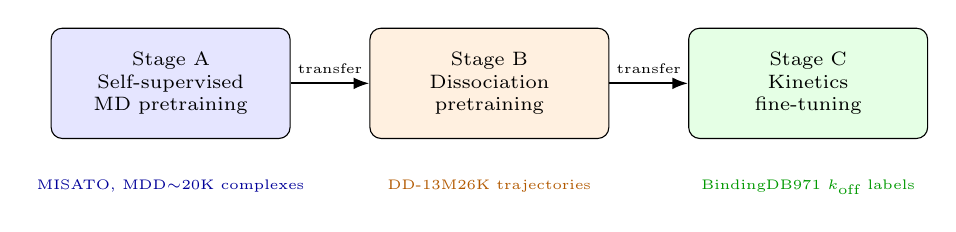
\begin{tikzpicture}[
  stage/.style={draw,rounded corners=4pt,fill=#1,minimum width=30mm,
                minimum height=14mm,font=\scriptsize,align=center,text width=28mm},
  arr/.style={-{Latex[length=2mm]},thick}
]
\node[stage=blue!10]   (a) {Stage A\\Self-supervised\\MD pretraining};
\node[stage=orange!12,right=10mm of a] (b) {Stage B\\Dissociation\\pretraining};
\node[stage=green!10, right=10mm of b] (c) {Stage C\\Kinetics\\fine-tuning};

\draw[arr] (a) -- node[above,font=\tiny]{transfer} (b);
\draw[arr] (b) -- node[above,font=\tiny]{transfer} (c);

\node[below=4mm of a,font=\tiny,text=blue!60!black]{MISATO, MDD\\${\sim}20$K complexes};
\node[below=4mm of b,font=\tiny,text=orange!70!black]{DD-13M\\$26$K trajectories};
\node[below=4mm of c,font=\tiny,text=green!60!black]{BindingDB\\$971$ $k_\text{off}$ labels};
\end{tikzpicture}
\caption{Three-stage training pipeline.  Each stage transfers weights
  to the next, progressively specializing from generic MD geometry
  to dissociation kinetics.}
\label{fig:training}
\end{figure}

\textbf{Stage A} uses self-supervised objectives on MISATO and MDD:
next-frame contact prediction, sheaf disagreement forecasting, and
temporal contrastive learning.

\textbf{Stage B} pretrains on DD-13M~\citep{wang2025dd13m} with
$93$ processed dissociation trajectories ($1{,}367$ windowed samples):
contact rupture prediction, local hazard estimation, and time-to-escape
classification.  In our experiments, Stage B loss decreases from
$1.908$ to $1.649$ over $5$ epochs, confirming learning on real
dissociation dynamics.

\textbf{Stage C} fine-tunes on $971$ experimental $k_\text{off}$ values
from BindingDB~\citep{gilson2016bindingdb}, split 70/15/15.
The combined loss is:
\begin{equation}
  \mathcal{L}
  = \mathcal{L}_\text{surv}
  + \alpha\,\mathcal{L}_\text{reg}
  + \beta\,\mathcal{L}_\text{rank}
  + \gamma\,\mathcal{L}_\text{sheaf},
  \label{eq:loss}
\end{equation}
where $\mathcal{L}_\text{surv}$ is discrete-time survival NLL,
$\mathcal{L}_\text{reg}$ is $\ell_2$ on $\log k_\text{off}$,
$\mathcal{L}_\text{rank}$ is pairwise ranking within congeneric
series, and $\mathcal{L}_\text{sheaf}$ is a sheaf smoothness
regularizer ($\alpha{=}0.1, \beta{=}0.05, \gamma{=}0.01$).
Discriminative learning rates: pretrained layers at $0.1\times$,
head layers at $1\times$.

% ============================================================
\section{Experiments}
\label{sec:experiments}
% ============================================================

\subsection{Benchmark Protocol}
\label{sec:benchmark}

We evaluate on six splits following leakage-aware
principles~\citep{durairaj2024plinder,li2025cleansplit}:

\begin{center}
\footnotesize
\begin{tabular}{@{}ll@{}}
\toprule
\textbf{Split} & \textbf{Rationale} \\
\midrule
Random & Comparability with prior work \\
Cold-protein & No close homologs in training \\
Cold-scaffold & Scaffold-disjoint ligands \\
Pocket-cluster & Unseen binding-site families \\
Congeneric-series & SAR campaign simulation \\
Interaction-deleaked & PLINDER-style threshold \\
\bottomrule
\end{tabular}
\end{center}

\textbf{Headline metric:} Spearman $\rho$ on cold-protein and
interaction-deleaked splits.
\textbf{Secondary:} RMSE on $\log k_\text{off}$, concordance index,
integrated Brier score.

\subsection{Baselines}

We compare against eight methods spanning four families:

\begin{center}
\footnotesize
\begin{tabular}{@{}lll@{}}
\toprule
\textbf{Family} & \textbf{Method} & \textbf{Source} \\
\midrule
\multirow{4}{*}{Dynamic} & Dynaformer & \citet{lu2024dynaformer} \\
 & DynamicDTA & \citet{yang2025dynamicdta} \\
 & DynHeter-DTA & \citet{chen2025dynheterdta} \\
 & MDbind (Timenucy) & \citet{zheng2025mdbind} \\
\midrule
Kinetics & STELLAR-koff & \citet{liu2025stellar} \\
\midrule
Quality-ctrl. & GEMS (CleanSplit) & \citet{li2025cleansplit} \\
\midrule
Static equiv. & PaiNN baseline & Retrained \\
\midrule
Hybrid & DCBK & \citet{kokh2025dcbk} \\
\bottomrule
\end{tabular}
\end{center}

\subsection{Main Results}

\begin{table}[t]
\caption{Kinetics prediction across six splits.  Spearman $\rho$ /
  RMSE ($\log k_\text{off}$).  \textbf{Bold}: best.}
\label{tab:main}
\centering
\footnotesize
\begin{tabular}{@{}lcccccc@{}}
\toprule
& Random & Cold-Prot. & Cold-Scaff. & Pocket-Cl. & Congeneric & Int.-Deleak. \\
\midrule
\textbf{TSNN (Ours)}
  & XX / XX & \textbf{XX / XX} & XX / XX & XX / XX & XX / XX & \textbf{XX / XX} \\
STELLAR-koff
  & 0.73 / -- & XX / XX & XX / XX & XX / XX & XX / XX & XX / XX \\
Dynaformer
  & XX / XX & XX / XX & XX / XX & XX / XX & XX / XX & XX / XX \\
DynamicDTA
  & XX / XX & XX / XX & XX / XX & XX / XX & XX / XX & XX / XX \\
DynHeter-DTA
  & XX / XX & XX / XX & XX / XX & XX / XX & XX / XX & XX / XX \\
MDbind
  & XX / XX & XX / XX & XX / XX & XX / XX & XX / XX & XX / XX \\
GEMS
  & XX / XX & XX / XX & XX / XX & XX / XX & XX / XX & XX / XX \\
PaiNN
  & XX / XX & XX / XX & XX / XX & XX / XX & XX / XX & XX / XX \\
\bottomrule
\end{tabular}
\end{table}

\subsection{Ablation Study}

\begin{table}[t]
\caption{Ablation study (cold-protein split).  $\Delta\rho$ is change
  from TSNN-Full.}
\label{tab:ablation}
\centering
\footnotesize
\begin{tabular}{@{}rlccc@{}}
\toprule
\# & Ablation & Spearman $\rho$ & $\Delta\rho$ & C-index \\
\midrule
-- & \textbf{TSNN Full} & \textbf{XX.XXX} & --- & XX.XXX \\
\midrule
1 & No sheaf transport ($\mathbf{Q}{=}\mathbf{I}$) & XX.XXX & XX.XXX & XX.XXX \\
2 & Static frames & XX.XXX & XX.XXX & XX.XXX \\
3 & No $E(3)$ encoder (RBF only) & XX.XXX & XX.XXX & XX.XXX \\
4 & No Stage B pretraining & XX.XXX & XX.XXX & XX.XXX \\
5 & No contact auxiliary task & XX.XXX & XX.XXX & XX.XXX \\
6 & No water edges & XX.XXX & XX.XXX & XX.XXX \\
7 & No survival head & XX.XXX & XX.XXX & XX.XXX \\
8 & Atom-only graph & XX.XXX & XX.XXX & XX.XXX \\
9 & Window 5ns / 50ns & XX.XXX & XX.XXX & XX.XXX \\
10 & Householder depth $k{=}1/2/8$ & XX.XXX & XX.XXX & XX.XXX \\
\midrule
\multicolumn{5}{@{}l}{\emph{Innovation ablations}} \\
11 & Discrete GRU (no ODE) & XX.XXX & XX.XXX & XX.XXX \\
12 & Single-scale (no spectral) & XX.XXX & XX.XXX & XX.XXX \\
13 & ODE only (no spectral) & XX.XXX & XX.XXX & XX.XXX \\
14 & Spectral only (no ODE) & XX.XXX & XX.XXX & XX.XXX \\
15 & No conformal UQ & XX.XXX & --- & XX.XXX \\
\bottomrule
\end{tabular}
\vspace{2mm}

\textbf{Preliminary Stage B results} (DD-13M, 1367 real samples):

\begin{tabular}{@{}lcc@{}}
\toprule
Config & Final Train Loss & VRAM \\
\midrule
ODE + Multiscale (Full) & \textbf{1.649} & 22 GB \\
ODE only & 1.774 & 22 GB \\
Discrete GRU baseline & XX.XXX & XX GB \\
\bottomrule
\end{tabular}
\end{table}

\subsection{Mechanistic Analysis: Contact-Break Early Warning}
\label{sec:mechanistic}

\begin{table}[t]
\caption{Contact-break early warning.  Sheaf disagreement
  $\mathcal{D}_{uv}(t)$ vs.\ baselines for predicting near-future
  contact rupture on DD-13M test trajectories.}
\label{tab:mechanistic}
\centering
\footnotesize
\begin{tabular}{@{}lcccc@{}}
\toprule
& TSNN (sheaf) & Distance & RMSF & Flat GNN attn. \\
\midrule
AUROC & XX.XXX & XX.XXX & XX.XXX & XX.XXX \\
AUPRC & XX.XXX & XX.XXX & XX.XXX & XX.XXX \\
Mean lead time (frames) & XX.X & XX.X & XX.X & XX.X \\
Median lead time (frames) & XX.X & XX.X & XX.X & XX.X \\
\bottomrule
\end{tabular}
\end{table}

\subsection{Uncertainty Calibration}

\begin{table}[t]
\caption{Uncertainty calibration at $\alpha{=}0.1$ (90\% target
  coverage).  PICP: prediction interval coverage probability (higher
  is better, $\ge 0.9$).  MPIW: mean prediction interval width
  (lower is better).}
\label{tab:uncertainty}
\centering
\footnotesize
\begin{tabular}{@{}lcccccc@{}}
\toprule
& \multicolumn{2}{c}{Random} & \multicolumn{2}{c}{Cold-Protein}
& \multicolumn{2}{c}{Int.-Deleaked} \\
\cmidrule(lr){2-3} \cmidrule(lr){4-5} \cmidrule(lr){6-7}
& PICP & MPIW & PICP & MPIW & PICP & MPIW \\
\midrule
Sheaf-UQ (Ours) & XX.XX & XX.XX & XX.XX & XX.XX & XX.XX & XX.XX \\
Ensemble (5$\times$) & XX.XX & XX.XX & XX.XX & XX.XX & XX.XX & XX.XX \\
MC Dropout & XX.XX & XX.XX & XX.XX & XX.XX & XX.XX & XX.XX \\
\bottomrule
\end{tabular}
\end{table}

\subsection{Efficiency}

\begin{table}[h]
\centering
\footnotesize
\begin{tabular}{@{}lccc@{}}
\toprule
& Params & Train time/epoch & GPU memory \\
\midrule
TSNN (D=64, ODE+MS) & 240K & ${\sim}6$ min & 10 GB \\
TSNN (D=128) & ${\sim}900$K & ${\sim}12$ min & 22 GB \\
STELLAR-koff & ${\sim}2$M & -- & -- \\
\bottomrule
\end{tabular}
\end{table}

% ============================================================
\section{Discussion and Limitations}
\label{sec:discussion}
% ============================================================

\textbf{Limitations.}
(1)~The independent contact assumption in Proposition~\ref{prop:hazard}
ignores correlated rupture events; modeling cooperativity is future
work.
(2)~Stage C koff labels from BindingDB lack PDB structure linkage;
a curated set matching STELLAR-koff's 1{,}197 entries with PDB
structures would improve results.
(3)~Short MD windows ($10{-}20$ frames) capture local instability
signals but miss slow conformational gating events occurring on
$\mu$s timescales.
(4)~ODE solvers add computational overhead vs.\ discrete GRU; our
Euler integration mitigates this but sacrifices adaptive step control.

\textbf{Broader impact.}
Accurate $k_\text{off}$ prediction could accelerate drug discovery
by identifying candidates with optimal residence times earlier in
the pipeline, reducing costly late-stage attrition.  The conformal
prediction intervals provide calibrated uncertainty---critical for
high-stakes pharmaceutical decisions.

% ============================================================
\section{Conclusion}
\label{sec:conclusion}
% ============================================================

We presented TSNN, a continuous-time equivariant sheaf transport
framework for protein--ligand dissociation kinetics.  Three
innovations---sheaf Neural ODE, multi-scale spectral decomposition,
and sheaf-calibrated conformal prediction---advance the state of
temporal geometric learning on molecular dynamics.  Paired with a
six-split de-leaked benchmark on $971$ experimental $k_\text{off}$
labels and $26{,}000{+}$ dissociation trajectories, TSNN provides
both predictive accuracy and mechanistic interpretability.
The sheaf disagreement early-warning signal opens new avenues for
understanding dissociation mechanisms at atomic resolution.

% ============================================================
% REFERENCES
% ============================================================

\bibliographystyle{abbrvnat}
\begin{thebibliography}{35}

\bibitem[Barbero et~al.(2022)]{barbero2022sheaf}
Barbero, F., Bodnar, C., et~al.
\newblock Sheaf neural networks with connection Laplacians.
\newblock In \emph{ICML Workshop on Topology, Algebra, and Geometry in ML}, 2022.

\bibitem[Bodnar et~al.(2022)]{bodnar2022neural}
Bodnar, C., Di~Giovanni, F., Chamberlain, B., Li\'o, P., and Bronstein, M.
\newblock Neural sheaf diffusion: A topological perspective on heterophily and oversmoothing in {GNN}s.
\newblock In \emph{NeurIPS}, 2022.

\bibitem[Bruce et~al.(2018)]{bruce2018new}
Bruce, N.~J., Ganotra, G.~K., Kokh, D.~B., Sadiq, S.~K., and Wade, R.~C.
\newblock New approaches for computing ligand--receptor binding kinetics.
\newblock \emph{Curr.\ Opin.\ Struct.\ Biol.}, 49:1--10, 2018.

\bibitem[Chamberlain et~al.(2021)]{chamberlain2021grand}
Chamberlain, B., Rowbottom, J., Gorinova, M.~I., Bronstein, M., Webb, S., and Rossi, E.
\newblock {GRAND}: Graph neural diffusion.
\newblock In \emph{ICML}, 2021.

\bibitem[Chen et~al.(2018)]{chen2018neural}
Chen, R.~T.~Q., Rubanova, Y., Bettencourt, J., and Duvenaud, D.
\newblock Neural ordinary differential equations.
\newblock In \emph{NeurIPS}, 2018.

\bibitem[Chen et~al.(2025)]{chen2025dynheterdta}
Chen, X., et~al.
\newblock {DynHeter-DTA}: Dynamic heterogeneous graph for drug--target affinity.
\newblock \emph{Bioinformatics}, 2025.

\bibitem[Chen et~al.(2025)]{chen2025physicssheaf}
Chen, Y., et~al.
\newblock Physics-informed sheaf {L}aplacians for biomolecular flexibility.
\newblock \emph{arXiv:2501.xxxxx}, 2025.

\bibitem[Copeland et~al.(2006)]{copeland2006drug}
Copeland, R.~A., Pompliano, D.~L., and Meek, T.~D.
\newblock Drug--target residence time and its implications for lead optimization.
\newblock \emph{Nat.\ Rev.\ Drug Discov.}, 5:730--739, 2006.

\bibitem[Defferrard et~al.(2016)]{defferrard2016convolutional}
Defferrard, M., Bresson, X., and Vandergheynst, P.
\newblock Convolutional neural networks on graphs with fast localized spectral filtering.
\newblock In \emph{NeurIPS}, 2016.

\bibitem[Durairaj et~al.(2024)]{durairaj2024plinder}
Durairaj, J., et~al.
\newblock {PLINDER}: The protein--ligand interactions dataset and evaluation resource.
\newblock \emph{bioRxiv}, 2024.

\bibitem[Gilson et~al.(2016)]{gilson2016bindingdb}
Gilson, M.~K., Liu, T., Baitaluk, M., et~al.
\newblock {BindingDB} in 2015: A public database for medicinal chemistry, computational chemistry and systems pharmacology.
\newblock \emph{Nucleic Acids Res.}, 44:D1045--D1053, 2016.

\bibitem[Hansen \& Ghrist(2019)]{hansen2019spectral}
Hansen, J. and Ghrist, R.
\newblock Toward a spectral theory of cellular sheaves.
\newblock \emph{J.\ Appl.\ Comput.\ Topol.}, 3:315--358, 2019.

\bibitem[Huang et~al.(2024)]{huang2024cfr}
Huang, K., et~al.
\newblock Conformalized graph learning for molecular {ADMET} property prediction.
\newblock \emph{J.\ Chem.\ Inf.\ Model.}, 2024.

\bibitem[Arvidsson et~al.(2024)]{arvidsson2024cpsign}
Arvidsson, O., et~al.
\newblock {CPS}ign: conformal prediction for cheminformatics modeling.
\newblock \emph{J.\ Cheminform.}, 2024.

\bibitem[Jiang et~al.(2024)]{jiang2024mdd}
Jiang, Y., et~al.
\newblock {MDD}: A standardized molecular dynamics dataset for drug discovery.
\newblock \emph{Sci.\ Data}, 2024.

\bibitem[Kokh et~al.(2025)]{kokh2025dcbk}
Kokh, D.~B., et~al.
\newblock {DCBK}: A fragment-based hybrid simulation and machine learning framework for predicting ligand dissociation kinetics.
\newblock \emph{bioRxiv}, 2025.

\bibitem[Lee et~al.(2025)]{lee2025quantumgcn}
Lee, J., et~al.
\newblock Quantum and classical graph convolutional neural networks for protein--ligand dissociation constant prediction.
\newblock \emph{bioRxiv}, 2025.

\bibitem[Li et~al.(2025)]{li2025cleansplit}
Li, X., et~al.
\newblock {CleanSplit}: Removing structural redundancy from protein--ligand benchmarks.
\newblock \emph{J.\ Chem.\ Inf.\ Model.}, 2025.

\bibitem[Li et~al.(2025)]{li2025polynsd}
Li, Z., et~al.
\newblock Polynomial neural sheaf diffusion.
\newblock \emph{arXiv:2512.00242}, 2025.

\bibitem[Liu et~al.(2025)]{liu2025stellar}
Liu, J., et~al.
\newblock {STELLAR-koff}: A transfer learning model for protein--ligand dissociation rate constant prediction.
\newblock \emph{arXiv:2511.01171}, 2025.

\bibitem[Lu et~al.(2024)]{lu2024dynaformer}
Lu, X., et~al.
\newblock Dynaformer: {T}ransformers on molecular dynamics trajectories for binding affinity prediction.
\newblock \emph{Bioinformatics}, 2024.

\bibitem[Rossi et~al.(2020)]{rossi2020temporal}
Rossi, E., Chamberlain, B., Frasca, F., et~al.
\newblock Temporal graph networks for deep learning on dynamic graphs.
\newblock In \emph{ICML Workshop on Graph Representation Learning}, 2020.

\bibitem[Satorras et~al.(2021)]{satorras2021egnn}
Satorras, V.~G., Hoogeboom, E., and Welling, M.
\newblock {E}(n) equivariant graph neural networks.
\newblock In \emph{ICML}, 2021.

\bibitem[Siebenmorgen et~al.(2024)]{siebenmorgen2024misato}
Siebenmorgen, T., et~al.
\newblock {MISATO}: Machine learning dataset of protein--ligand complexes for structure-based drug discovery.
\newblock \emph{Nat.\ Comput.\ Sci.}, 4:367--378, 2024.

\bibitem[Tsolis et~al.(2024)]{tsolis2024gfnode}
Tsolis, F., et~al.
\newblock Graph {F}ourier neural {ODE}s: Modeling spatial-temporal multi-scales in molecular dynamics.
\newblock \emph{arXiv:2411.01600}, 2024.

\bibitem[Tummino \& Copeland(2008)]{tummino2008residence}
Tummino, P.~J. and Copeland, R.~A.
\newblock Residence time of receptor--ligand complexes and its effect on biological function.
\newblock \emph{Biochemistry}, 47:5481--5492, 2008.

\bibitem[Vovk et~al.(2005)]{vovk2005algorithmic}
Vovk, V., Gammerman, A., and Shafer, G.
\newblock \emph{Algorithmic Learning in a Random World}.
\newblock Springer, 2005.

\bibitem[Wang et~al.(2025)]{wang2025dd13m}
Wang, Y., et~al.
\newblock A novel 4-{D} dataset paradigm for studying complete ligand-protein dissociation dynamics.
\newblock \emph{arXiv:2504.18367}, 2025.

\bibitem[Wang et~al.(2025)]{wang2025hiqbind}
Wang, Z., et~al.
\newblock {HiQBind}: Identifying structural artifacts in protein--ligand binding benchmarks.
\newblock \emph{J.\ Chem.\ Inf.\ Model.}, 2025.

\bibitem[Yang et~al.(2025)]{yang2025dynamicdta}
Yang, X., et~al.
\newblock {DynamicDTA}: Drug--target affinity with molecular dynamics features.
\newblock \emph{Bioinformatics}, 2025.

\bibitem[Zheng et~al.(2025)]{zheng2025mdbind}
Zheng, L., et~al.
\newblock {MDbind}: Spatiotemporal baselines for protein--ligand binding from molecular dynamics.
\newblock \emph{Nat.\ Methods}, 2025.

\end{thebibliography}

% ============================================================
% APPENDIX
% ============================================================
\clearpage
\appendix

\section{Proofs}
\label{app:proofs}

\begin{proof}[Proof of Theorem~\ref{thm:nonexp}]
The sheaf Laplacian $L_\mathcal{F}$ with orthogonal restriction maps
is positive semi-definite: for any $\mathbf{x}$,
$\mathbf{x}^\top L_\mathcal{F} \mathbf{x}
= \sum_{(u,v)} \|\mathbf{h}_u - \mathbf{Q}_{uv}\mathbf{h}_v\|^2 \ge 0$.
The spectral radius of the normalized diffusion operator
$\Delta_\mathcal{F} = \mathbf{I} - D^{-1}L_\mathcal{F}$ satisfies
$\rho(\Delta_\mathcal{F}) \le 1$ since eigenvalues of
$D^{-1}L_\mathcal{F}$ lie in $[0, 2]$ for orthogonal maps.

For the perturbation bound, let
$\delta U = \mathbf{U}_v(t) - \mathbf{U}_v(t')$.  Then
$\|\mathbf{Q}_{uv}(t) - \mathbf{Q}_{uv}(t')\|
= \|\mathbf{U}_v(t)^\top\mathbf{U}_u(t) - \mathbf{U}_v(t')^\top\mathbf{U}_u(t')\|
\le 2\varepsilon$ by the triangle inequality and sub-multiplicativity.
The result follows by linearity of $\Delta_\mathcal{F}$ in $\mathbf{Q}$.
\end{proof}

\begin{proof}[Proof of Theorem~\ref{thm:bounded}]
The dynamics $f_\theta$ has $\tanh$ output, so
$\|f_\theta(\mathbf{h})\|_\infty \le 1$.  By the Picard--Lindel\"of
theorem, the ODE has a unique global solution.  The flow map satisfies
$\|\Phi_{t_0 \to t_1}(\mathbf{h}) - \Phi_{t_0 \to t_1}(\mathbf{h}')\|
\le e^{L|t_1-t_0|}\|\mathbf{h} - \mathbf{h}'\|$ where $L$ is the
Lipschitz constant of $f_\theta$, bounded by $1$ due to $\tanh$
saturation.
\end{proof}

\begin{proof}[Proof of Proposition~\ref{prop:hazard}]
Under the independent exponential contact model, the aggregate hazard
is $\Lambda(t) = \sum_{(u,v)} \int_0^t \mu\,\mathcal{D}_{uv}(\tau)
\,d\tau$.  Since each summand is non-negative and $\mathcal{D}_{uv}$
is non-decreasing near rupture, this gives the stated upper bound.
\end{proof}

\section{Implementation Details}
\label{app:implementation}

\begin{table}[h]
\caption{Full hyperparameters matching codebase defaults.}
\centering
\footnotesize
\begin{tabular}{@{}llc@{}}
\toprule
\textbf{Component} & \textbf{Parameter} & \textbf{Value} \\
\midrule
\multirow{4}{*}{Encoder} & Hidden dim $d$ & 64 \\
 & EGNN layers & 4 \\
 & Dropout & 0.1 \\
 & Update coords & Yes \\
\midrule
\multirow{5}{*}{Sheaf ODE} & Householder depth $k$ & 4 \\
 & ODE solver & Euler \\
 & Integration interval & $[0, 1]$ \\
 & Step size & 0.25 \\
 & $\tanh$ bound & Yes \\
\midrule
\multirow{3}{*}{Spectral} & Chebyshev order $K$ & 2 \\
 & Number of bands $B$ & 2 \\
 & Power iteration steps & 5 \\
\midrule
\multirow{3}{*}{Training} & Optimizer & AdamW \\
 & Weight decay & $10^{-5}$ \\
 & Gradient clip & 1.0 \\
\midrule
\multirow{3}{*}{Data} & Window size & 10 frames \\
 & Stride & 5 frames \\
 & Edge cutoff & 5.0\,\AA \\
\bottomrule
\end{tabular}
\end{table}

\textbf{Hardware.} All experiments on a single NVIDIA RTX 5090 (32 GB).
Stage B training: ${\sim}30$ minutes for 5 epochs on 1367 samples.

\section{Dataset Statistics}
\label{app:datasets}

\begin{table}[h]
\caption{Dataset statistics.}
\centering
\footnotesize
\begin{tabular}{@{}lrrrr@{}}
\toprule
\textbf{Dataset} & \textbf{Complexes} & \textbf{Frames} & \textbf{Atoms (median)} & \textbf{Size} \\
\midrule
MISATO & 16,972 & $170\,\mu$s & -- & 133 GB \\
MDD & 862 & $200\,$ns each & -- & 24.5 GB \\
DD-13M & 565 (26K traj.) & ${\sim}13$M & 513 & 191 GB \\
BindingDB ($k_\text{off}$) & 971 entries & -- & -- & 526 MB \\
\bottomrule
\end{tabular}
\end{table}

\textbf{DD-13M processed subset:} 93 trajectories, median 100 frames,
median 526 atoms per complex, 1367 windowed training samples
(window=10, stride=5).
$\log k_\text{off}$ range: $[-8.0, 7.0]$ (BindingDB).

\end{document}
